\section{Genome Projects}
\subsection{Entelegyne Spider}

  Citation \cite{carlson_novo_2015}

  ``In this study, the transcriptomes of six entelegyne spider species from
  three genera (\textit{Cicurina travisae}, \textit{C. vibora},
  \textit{Habronattus signatus}, \textit{H. ustulatus}, \textit{Nesticus
    bishopi} and \textit{N.  cooperi}) were sequenced and de novo assembled
  \dots between ~ 400 and 1,100 unique orphan genes were found to be present in
  each congeneric lineage''

\subsection{Potato blight \textit{Phytophthora infestans}}

  Citation \cite{haas_genome_2009}

  Genome is arragned into two sets of blocks: 1) gene-rich, synteny-conserved
  blocks and 2) gene-poor, repeat-rich, TE-rich, and secreted-effector-rich
  blocks.

  $~$1/3 of the genome is comprised of Gypsy elements.

  Some fungal motifs effectors are conserved, such as the huge RXLR (563, half
  species-specific) and Crinkler (CRN) families of cytoplasmic effectors
  \cite{haas_genome_2009}. The RXLR effectors where identified via HMM against
  known motifs, however, at the unweighted sequence level, half were
  species-specific. Only 16/563 where present in all three sequenced species of
  the genus. These genes had extremely fast turnover rate. Markov clustering
  (TribalMCL) show 1 large family and 150 smaller ones. The RXLR genes are
  mostly in the gene-sparse blocks, where transposons can hasten evolution.

  CRN cytoplasmic effectors have a conserved N-terminal $~$50 aa LFLAK domain
  and highly variable C-terminal domain(s). They are concentrated in
  gene-sparse regions where they may rapidly recombine, shuffling the
  C-terminal domain into new sequences.

  The authors suggest non-allelic homologous recombination and tandem gene
  duplication as the primary methods of family expansion in RXLR and CRN.  They
  find no evidence of transposition.

  \begin{figure}[h!]
    \centering
    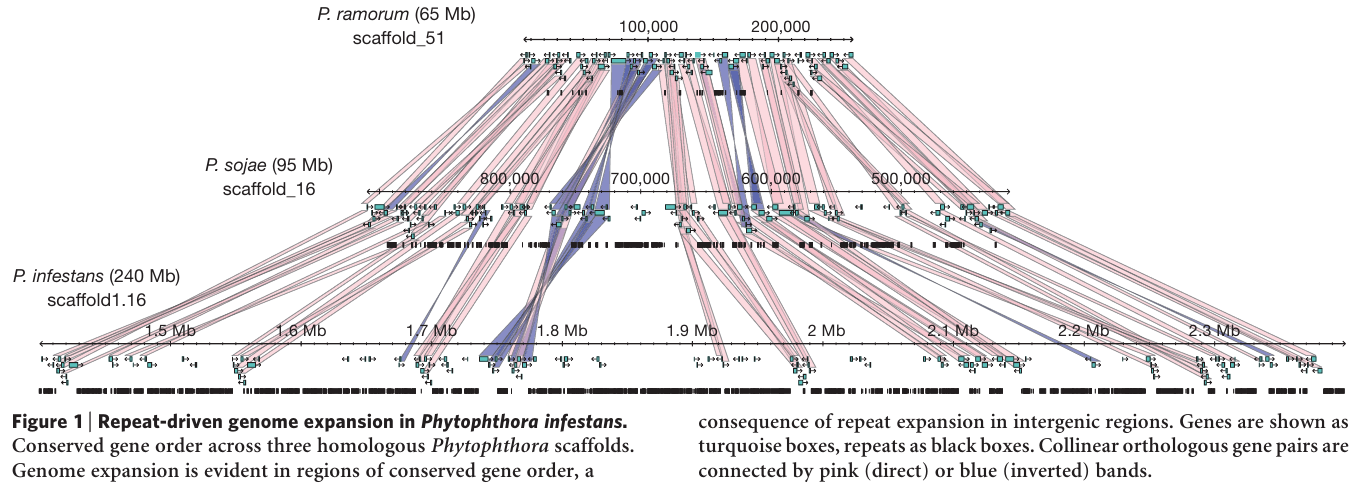
\includegraphics[width=\textwidth]{haas_blight_2009-fig1}
    \caption{
        Haas (2009) \cite{haas_genome_2009}
    }
  \end{figure}

  \begin{figure}[h!]
    \centering
    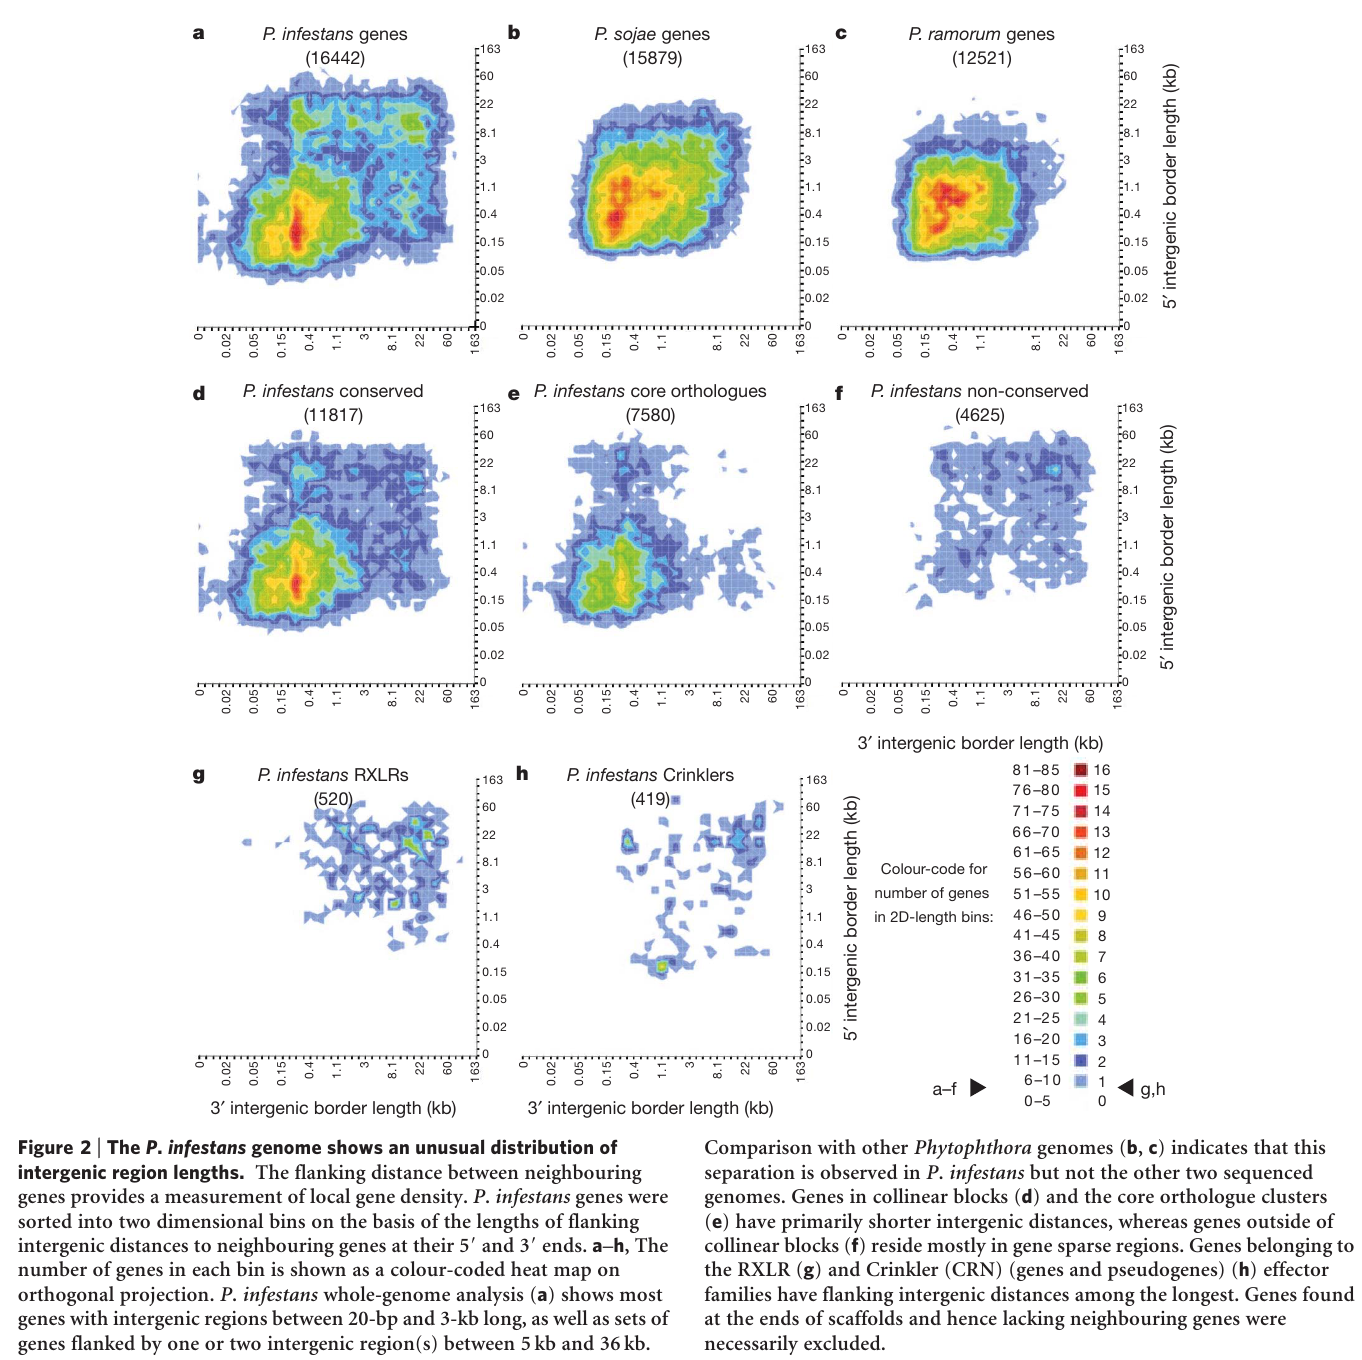
\includegraphics[width=\textwidth]{haas_blight_2009-fig2}
    \caption{
        Haas (2009) \cite{haas_genome_2009}
    }
  \end{figure}

  \begin{figure}[h!]
    \centering
    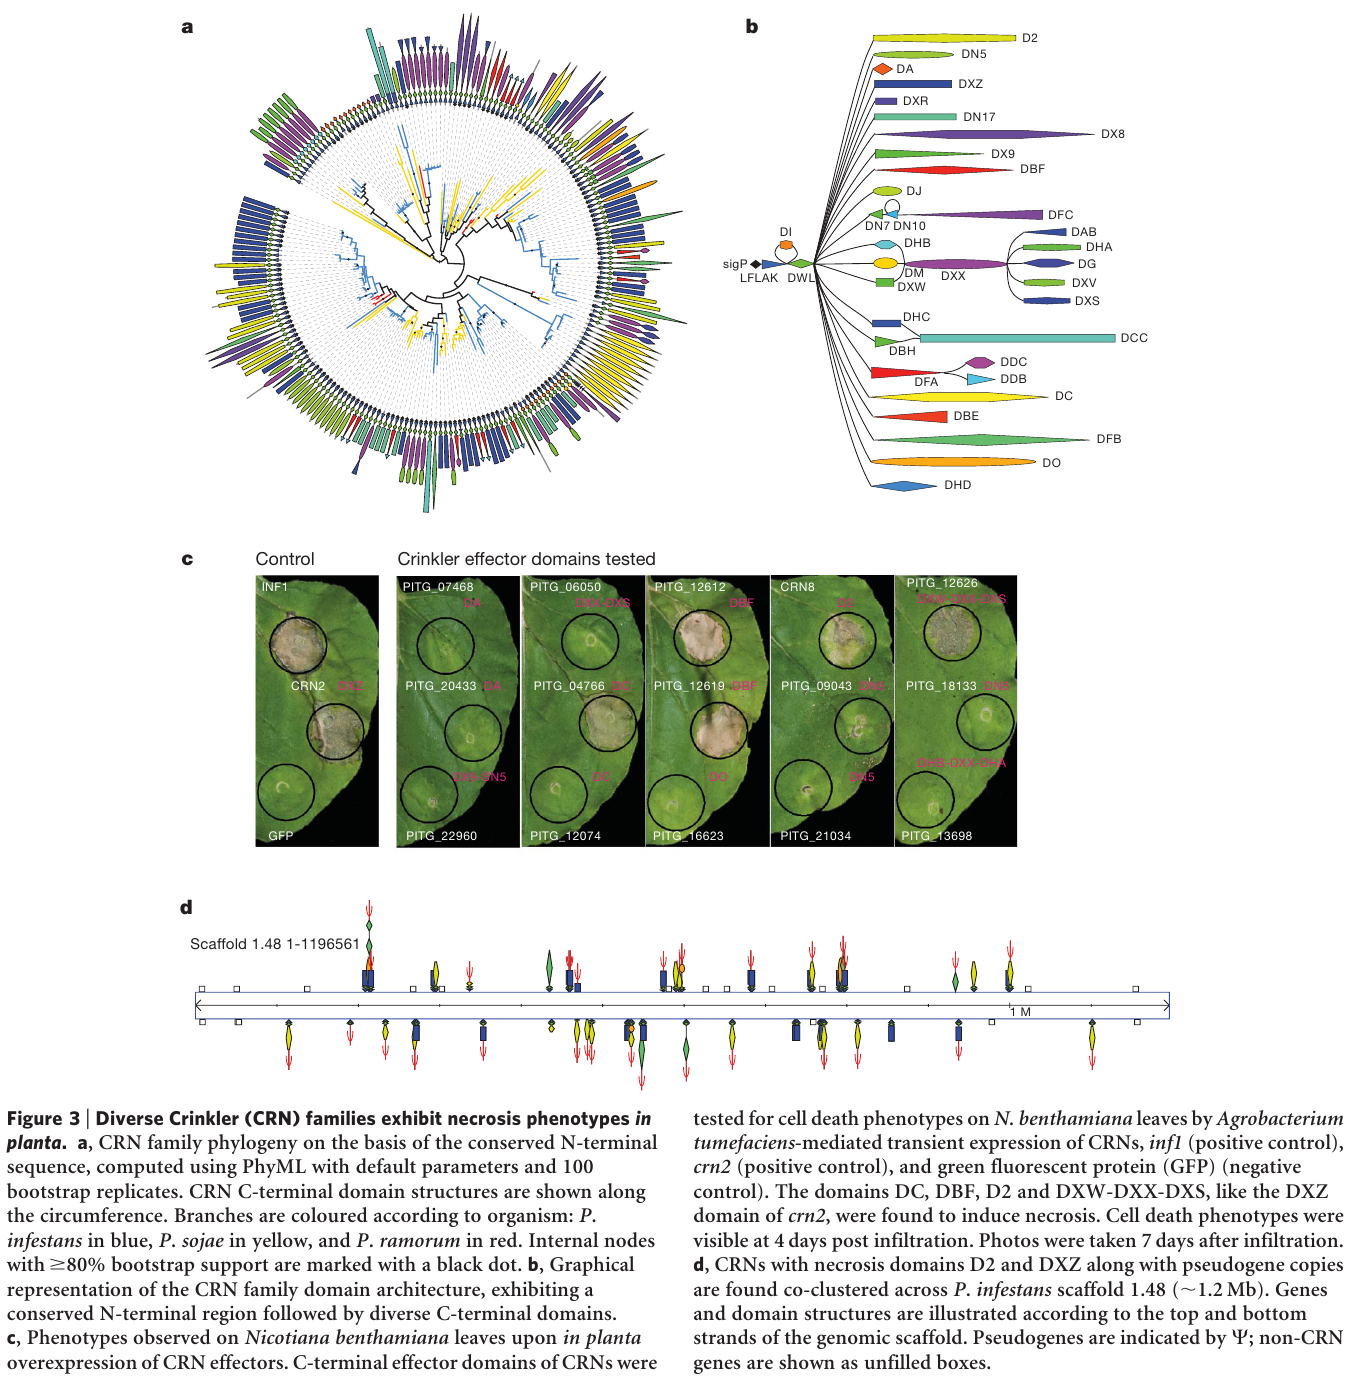
\includegraphics[width=\textwidth]{haas_blight_2009-fig3}
    \caption{
        Haas (2009) \cite{haas_genome_2009}
    }
  \end{figure}

  \FloatBarrier

\subsection{18 Dothideomycetes Fungi genomes}

  Citation \cite{ohm_diverse_2012}

  \begin{figure}[h!] \centering
    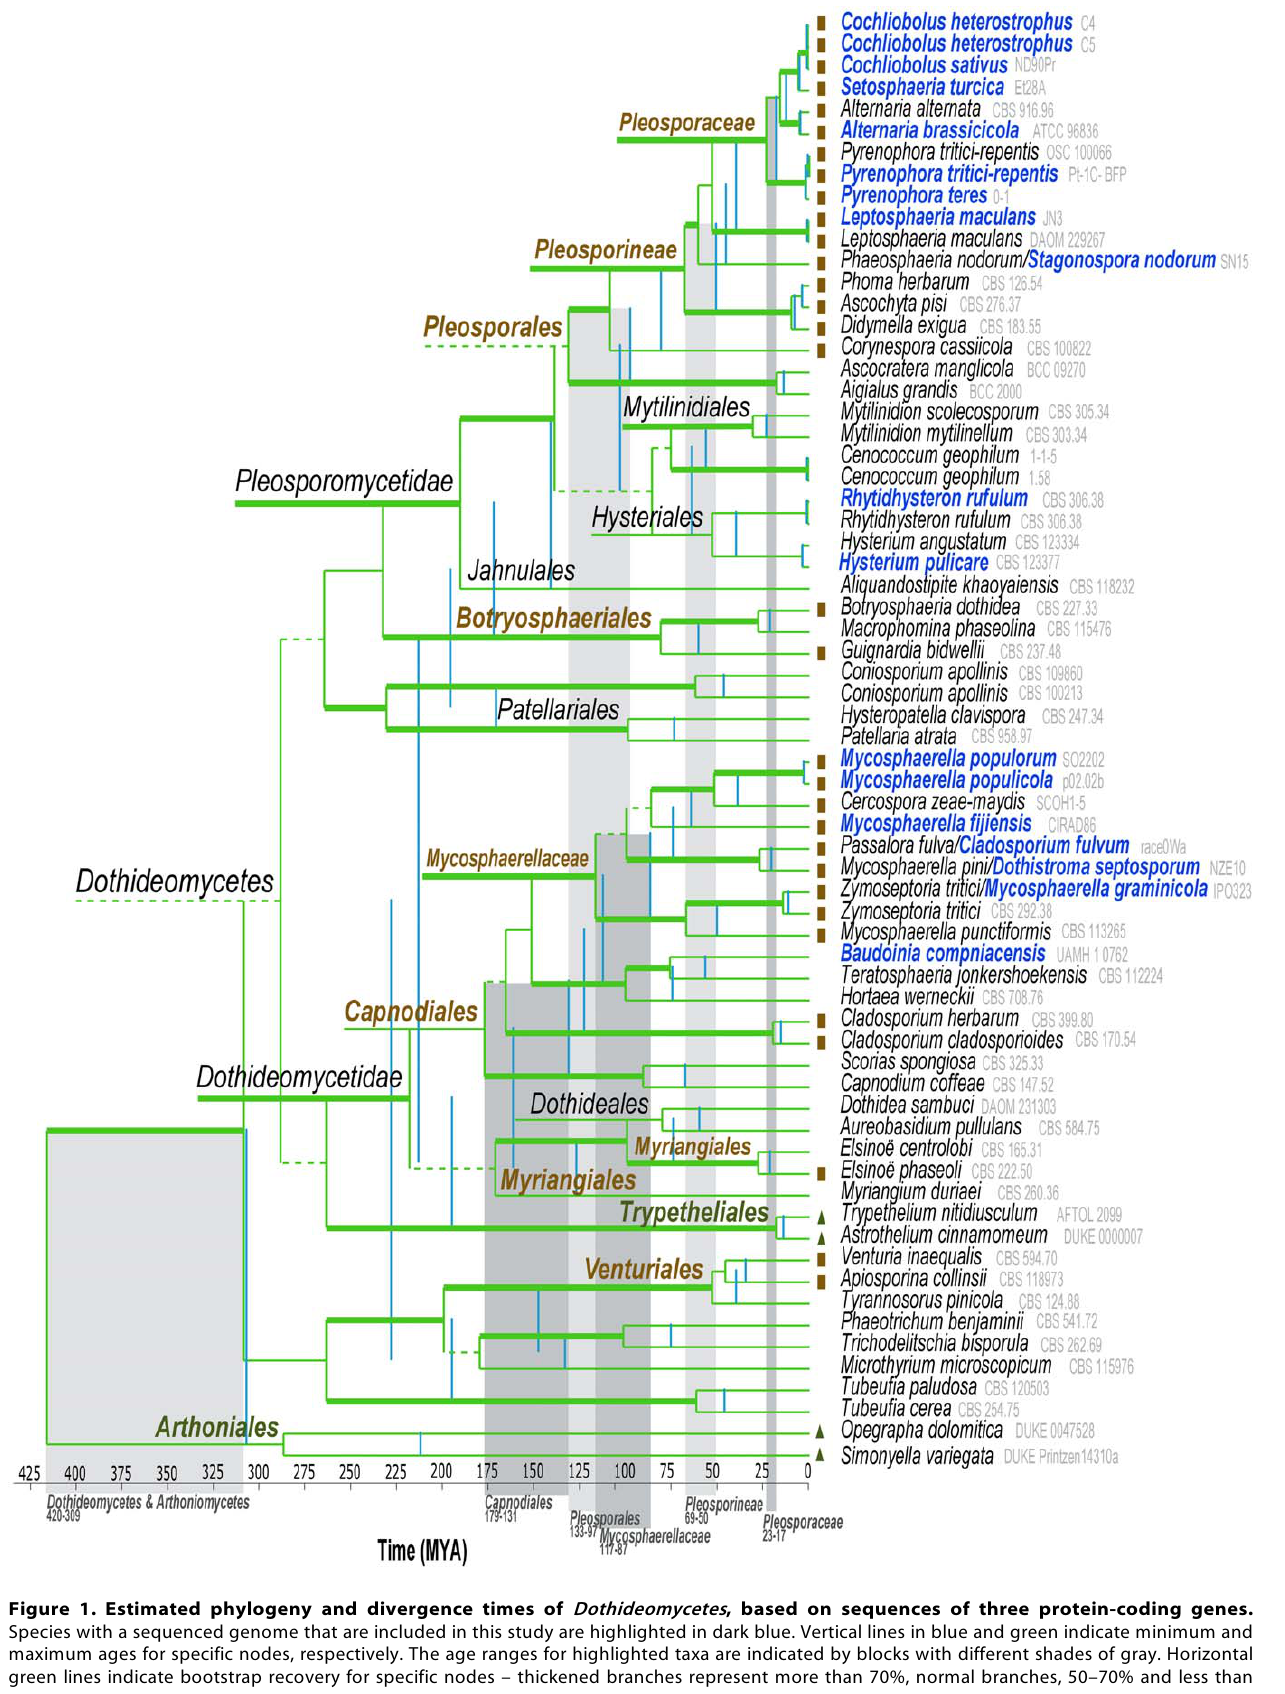
\includegraphics[height=0.7\textheight]{ohm_18fungi_2012-fig1}
  \end{figure}

  \begin{figure}[h!] \centering
    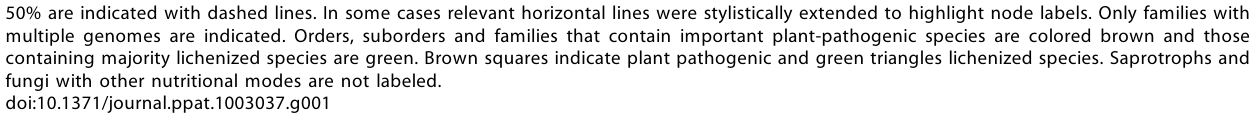
\includegraphics[width=0.7\textwidth]{ohm_18fungi_2012-fig1b}
    \caption{Ohm (2012) \cite{ohm_diverse_2012}}
  \end{figure}

  \begin{figure}[h!] \centering
    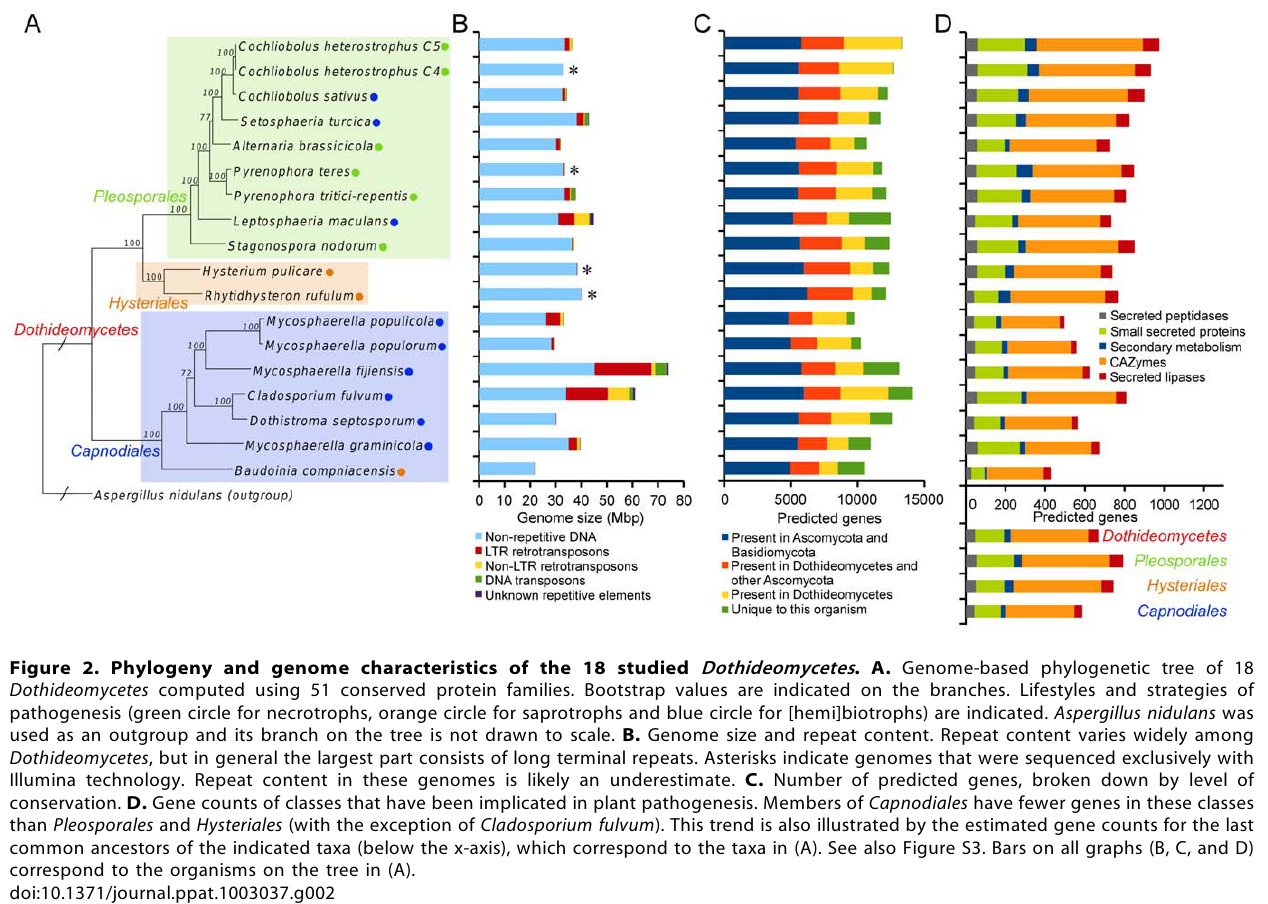
\includegraphics[width=\textwidth]{ohm_18fungi_2012-fig2}
    \caption{Ohm (2012) \cite{ohm_diverse_2012}}
  \end{figure}

  \begin{figure}[h!] \centering
    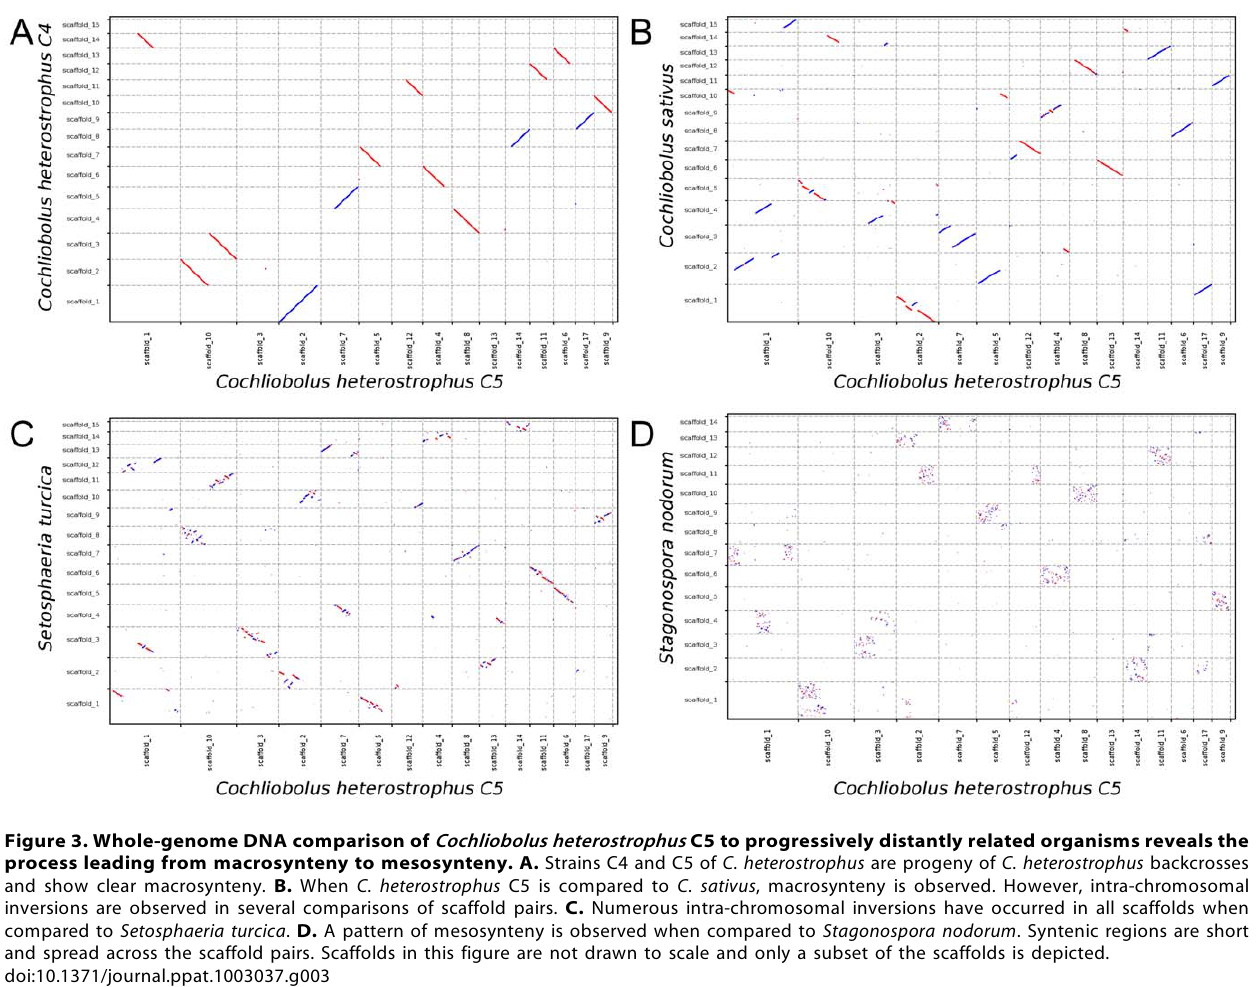
\includegraphics[width=\textwidth]{ohm_18fungi_2012-fig3}
    \caption{Ohm (2012) \cite{ohm_diverse_2012}}
  \end{figure}

  \FloatBarrier

\subsection{Setosphaeria fungi genome}

  Citation \cite{wu_setosphaeria_2013}

  \begin{figure}[h!] \centering
    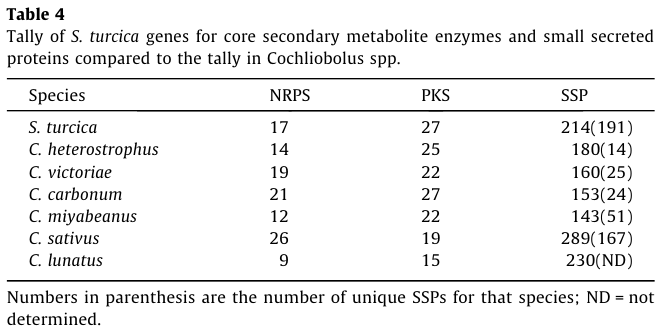
\includegraphics[width=0.6\textwidth]{wu_setosphaeria_2013-t1}
    \caption{Wu (2013) \cite{wu_setosphaeria_2013}}
  \end{figure}

  ``As reported in (Condon et al., 2013), candidate SSPs in S. turcica and
  nine Cochliobolus isolates were identified by screening gene catalogs for
  proteins smaller than 200 amino acids, containing more than 2\% cysteine,
  secretion signals, and lacking transmem- brane domains (Table 4).
  Cross-genome comparisons were made based on all vs. all reciprocal best hit
  analysis with an 80\% similarity cutoff (species-unique in parentheses).
  Note that both hemibio- trophs in this comparison, S. turcica and C.
  sativus, contained more strain unique SSPs than necrotrophs.'' pp. 4 (see
  table)

  \FloatBarrier
\subsection{Spanu (2010): Powdery Mildew \textit{ Blumeria graminis f.sp. hordei}}

  Citation \cite{spanu_genome_2010}

  No RIP, 64\% TE composition. Genes are clustered in little islands in the transposon sea.


  ``In addition to >1350 paralog copies of the previously described atypical
  avirulence genes AVRk1 and AVRa10 (11), we predicted 248 Blumeria proteins with
  a signal peptide (SP) but lacking any transmembrane domain and BLAST (Basic
  Local Alignment Search Tool) hit outside the mildews, thus representing
  candidates for secreted effector proteins (CSEPs) (12). The CSEPs have
  distinctive features (table S6) and show great sequence diversity with few
  members grouping in small families (Fig. 3A). We noted no obvious clustering of
  CSEPs within the Blumeria contigs. Approximately 80\% harbor a recently
  identified N-terminal tripeptide motif, termed “YxC,” (13), that typically
  occurs within the first 30 amino acids after the predicted SP cleavage site.
  Searches in the E. pisi and G. orontii genomes revealed that the vast majority
  of CSEPs are confined to Blumeria (Fig. 3A and table S6).  Thus, powdery mildew
  genomes preferentially harbor species- and/or tribe-specific innovations, which
  possibly evolved in the context of cospeciation with their plant hosts (11).
  Upon comparison of global gene expression in haustoria (Fig. 1C) and epiphytic
  structures (Fig. 1D), we observed preferential expression of the majority of
  the CSEPs (79\%) in haustoria (Fig. 3B), suggesting they have specific
  functions in biotrophic pathogenesis (14).'' pp. 4

  \begin{figure}[h!] \centering
    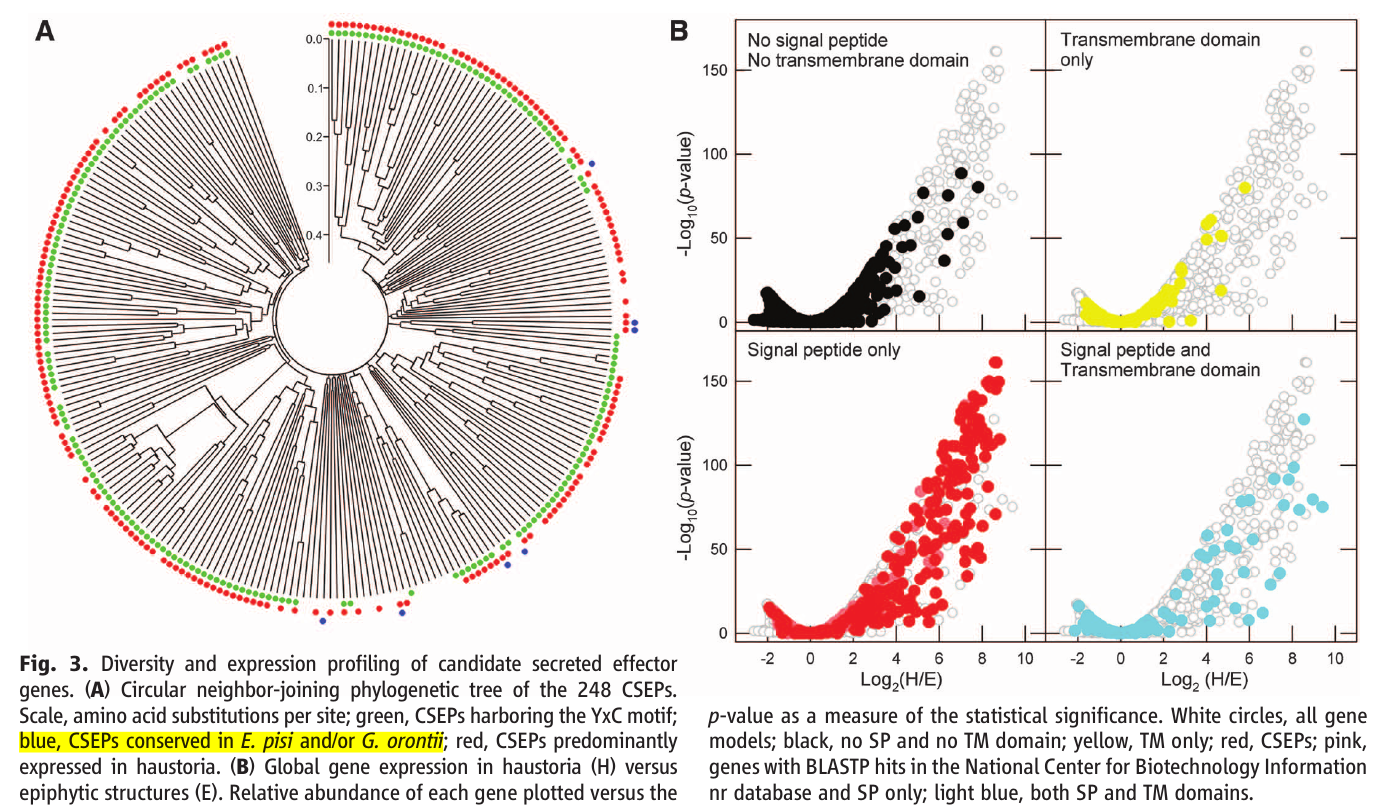
\includegraphics[width=\textwidth]{spanu_powder_2010-fig3}
    \caption{Spanu (2010) \cite{spanu_genome_2010}}
  \end{figure}
  \FloatBarrier

\subsection{Wicker (2013):Powdery Mildew \textit{ Blumeria graminis f.sp. tritici}}

  Citation \cite{wicker_wheat_2013}

  90\% transposable element (TE) composition

  The Blumeria graminis are divided into 8 \textit{formae speciales} that
  specifically infect a single host. tritici and hordei are estimated to be
  6.3 million years apart. 

  \begin{figure}[h!] \centering
    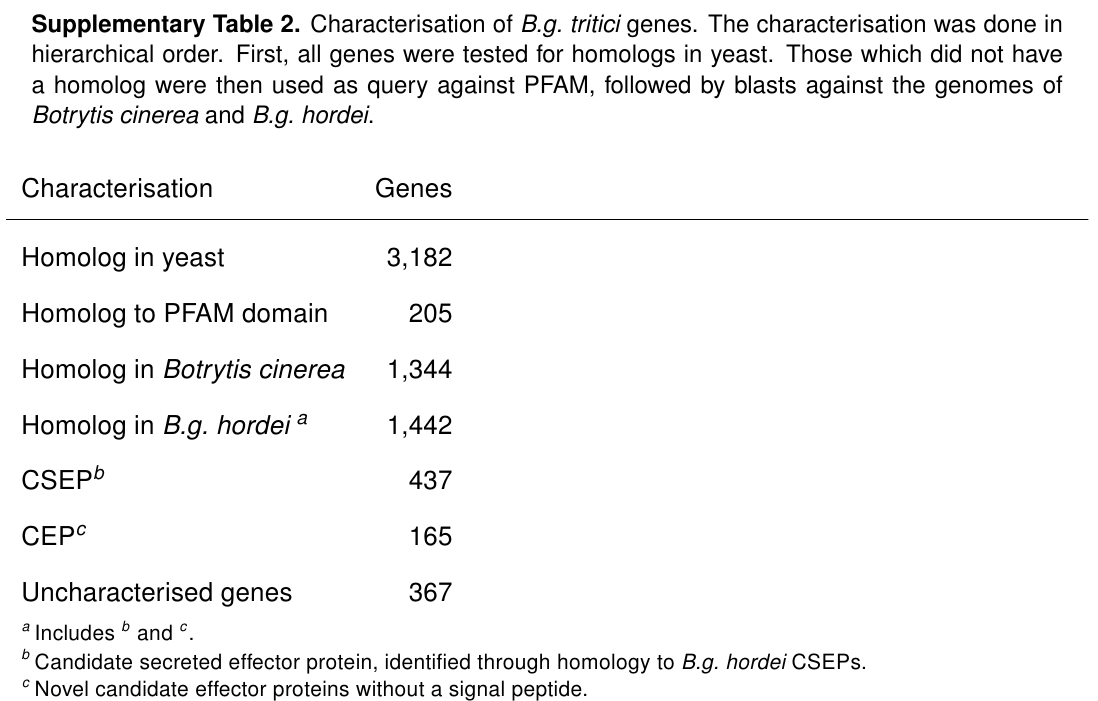
\includegraphics[width=0.7\textwidth]{wicker-rust-2013-suptab2}
    \caption{Wicker (2013) \cite{wicker_wheat_2013} It seems they didn't do thier own search for CSEPs}
  \end{figure}
  \FloatBarrier

  \begin{figure}[h!] \centering
    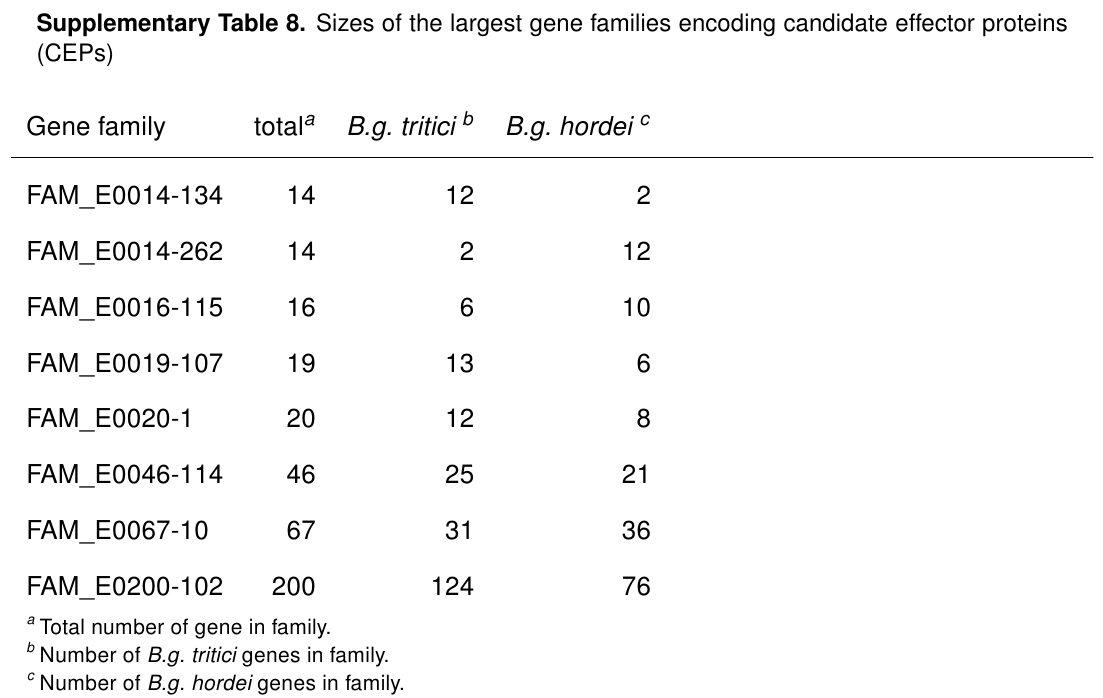
\includegraphics[width=0.7\textwidth]{wicker-rust-2013-suptab8}
    \caption{Wicker (2013) \cite{wicker_wheat_2013} }
  \end{figure}
  \FloatBarrier

  This is a shit paper. They didn't search for their own CSEPs in tritici,
  rather they identified CSEPs by looking for homologs in hordei.  They found
  437 CSEPs, while in hordei there are 248. So clearly there are major
  differences. But they didn't address this. Also they failed to mention
  which hordei CSEPs where \textit{not} present in tritici. So all we know is
  that at least one family of CSEPs is shared between the two sp.

  28\% of its genes had no homolog in Botrytis cinerea, seperate by 110 million years (TimeTree)

  Another annoying thing is that they find 92\% of the genes in tritici have
  a homolog in hordei. There conclusion is that the gene complement of the
  two subspecies is almost the same. In what universe is 8\% difference in
  gene content at a subspecies level \textit{almost the same}?

\subsection{Schnable (2009) B73 Maize}
  Citation \cite{schnable_b73_2009}

  \begin{figure}[h!] \centering
    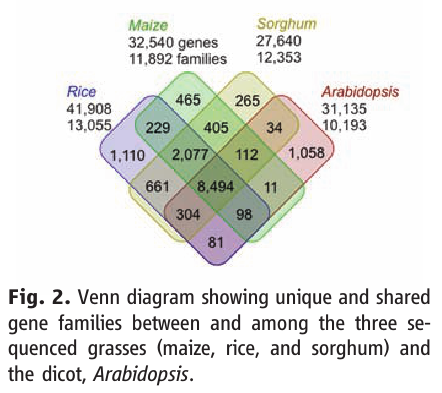
\includegraphics[width=0.3\textwidth]{schnable-maize-fig2}
    \caption{Schnable (2009) \cite{schnable_b73_2009}}
  \end{figure}
  \FloatBarrier
